\documentclass[11pt,a4paper]{article}
\usepackage[margin=2.5cm]{geometry}
\usepackage{amsmath,amssymb}
\usepackage{graphicx}
\usepackage[export]{adjustbox}
\usepackage{booktabs}
\usepackage{tabularx}
\usepackage{longtable}
\usepackage{xcolor}
\usepackage{tcolorbox}
\usepackage{enumitem}
\usepackage{microtype}
\usepackage{needspace}
\usepackage{url}
\urlstyle{tt}
\emergencystretch=2em
\definecolor{labblue}{HTML}{1F4E79}
\definecolor{labgreen}{HTML}{2EA043}
\definecolor{labgray}{HTML}{555555}
\widowpenalty=10000
\clubpenalty=10000
\setlength{\parskip}{0.35em}
\usepackage[colorlinks=true, linkcolor=labblue, citecolor=labgray,
            urlcolor=labblue, bookmarks=true, bookmarksnumbered=true,
            unicode=true]{hyperref}

\hypersetup{
    pdftitle={Chiral Protection (AIII): Why D7 Works and Where It Breaks},
    pdfauthor={Isaev, Iskhak Khamzatovich},
    pdfsubject={AB-Cloud Dirac Laboratory — per-test monograph D8},
    pdfkeywords={Dirac equation, Hofstadter model, Riemann zeta zeros, AB-Cloud, D8}
}
\begin{document}

\noindent{\small\color{labgray}\texttt{AB-Cloud Dirac Laboratory · per-test monograph · D8 · seed 96 · v1.4}}\\[0.3em]
\rule{\textwidth}{0.8pt}\\[0.6em]
{\LARGE\bfseries\color{labblue} Chiral Protection (AIII): Why D7 Works and Where It Breaks}\\[0.5em]
{\normalsize\itshape Test D8 — $\{H,\Gamma\} = 0$ exactly, $E \leftrightarrow -E$ to $4\times10^{-15}$ over 800 pairs}\\[0.4em]
\rule{\textwidth}{0.4pt}

\begin{tcolorbox}[colback=labgreen!8, colframe=labgreen!70!black, title={Verdict: PASS — 4/4 checks}, fonttitle=\bfseries, boxrule=0.6pt]
\textbf{Abstract.} Test D8 establishes the symmetry mechanism behind D7's verdicts: under the full $\zeta$-decoration the chiral (sublattice) anticommutator remains $\{H, \Gamma\} = 0$ \emph{exactly} -- not small, exactly -- and the spectrum is therefore pairwise symmetric, $E \leftrightarrow -E$ verified over 800 pairs to $4\times10^{-15}$. This AIII-type protection is what survives the decoration and what the transport and index results of D9--D13 build upon. What it does \emph{not} protect is the exact zero pinning of the clean tower: D8 measures the splitting of the tower into $\pm E$ valley pairs and documents the vanishing-index mechanism, turning D7's honest negative into a structural statement.
\end{tcolorbox}

\section{What This Test Verifies}
The clean $\pi$-flux lattice is bipartite: every hop connects opposite sublattices, so in the sublattice basis $H$ is purely off-diagonal and anticommutes with the chiral operator $\Gamma = \mathrm{diag}(+1, -1)$. This is the tenfold-way class AIII, and its spectral consequence is rigid: if $E$ is an eigenvalue so is $-E$, with eigenvectors of opposite $\Gamma$-polarity \cite{mecklenburgshen}. The vortex gauge of the parent construction acts on bond \emph{phases} only -- it never connects same-sublattice sites -- so the anticommutation is a structural identity, not a numerical accident. D8 verifies this directly on the decorated operator.

The same rigidity explains why the \emph{statistics} can move while the \emph{symmetry} cannot: complex bond phases change the phases of the off-diagonal blocks, feeding the GUE-complexifying ingredients that D7 measures, but they cannot produce a diagonal block and therefore cannot break the $\pm E$ pairing. The exact zero tower is a different story: pinning at $E = 0$ requires not just symmetry but an index -- a topological count of $\Gamma^+$ minus $\Gamma^-$ states in the zero subspace. Under the decoration the index vanishes (the count is balanced), and with it the protection of the pinning; the tower dissolves into valley pairs while the pairing law itself stays exact \cite{atyahbott}.

\section{Model and Method}
On the $L = 40$, $N_v = 44$ $\zeta$-decorated torus (the canonical size) the test computes: (i) the chiral anticommutator norm $\|\{H, \Gamma\}\|$ exactly in machine arithmetic; (ii) a full same-sublattice-hopping scan of the Hamiltonian matrix, which must return zero for bipartiteness; (iii) the pairwise spectral symmetry -- sorting $E$ and $-E$ and measuring the maximum deviation across all $\pm$ pairs; and (iv) the zero-mode content, reported with its chiral-multiplet consistency check. The pairing audit is the most demanding: at 1600 eigenvalues it involves 800 pairs and a tolerance of $10^{-10}$, measured against a machine-level outcome.

The companion figure turns the pairing law into pictures: a scatter of the pair deviation $|E_i + E_{\bar i}|$ against $|E_i|$ on a logarithmic axis, and the histogram of the same deviations, both recomputed at $L = 32$ with the canonical modules and seed. Every pair sits at machine depth -- the visual signature of a symmetry that is exact, not approximate.

\subsection{Parameters and conventions}
\begin{table}[htbp]\centering\small
\begin{tabularx}{\columnwidth}{@{}l l X@{}}
\toprule
Quantity & Value & Meaning \\
\midrule
Canonical size & $L = 40$, $N\_v = 44$ ($\zeta$-coded) & parent density rule \\
Chiral operator & $\Gamma = (-1)^{x+y}$ & sublattice basis \\
Pairing audit & $\max\_i |E\_i + E\_{\bar i}|$ over 800 pairs & tolerance $10^{-10}$ \\
Bipartite scan & same-sublattice hopping matrix entries & must be exactly 0 \\
Seed & 96 & deterministic \\
\bottomrule
\end{tabularx}
\caption{D8 parameters and conventions (seed 96, parent gauge constants).}
\end{table}

\section{Results}
All four audits return their ideal values: $\|\{H, \Gamma\}\| = 0.00\times10^{+0}$ exactly; the same-sublattice scan finds zero same-sublattice hopping; the pairing symmetry holds to $4.0\times10^{-15}$ across 800 pairs; and the zero-mode content ($n_0 = 0$ under decoration) is chiral-multiplet-consistent -- an even, balanced content, exactly what a vanishing index predicts. The AIII protection is thus verified as an exact structural property of the decorated operator.

The mechanism of D7's negative result is now explicit: the decoration preserves the symmetry (pairing) but destroys the clean-limit index (pinning). In the language of the tenfold way, the operator remains in class AIII where $\pm E$ pairing is symmetry-enforced, but the zero-pinning was never symmetry-enforced at index zero -- it was a translational (clean-limit) signature. This reading is what makes D9's index-restoration programme well posed: to restore protected zero modes one must supply a genuine index, which is precisely what a Jackiw--Rebbi--Rossi mass texture does \cite{jackiwrebbi,jackiwrossi}.

\subsection{Key numbers}
\begin{tcolorbox}[colback=labblue!6, colframe=labblue!70!black, boxrule=0.6pt, title={Key results (canonical run)}]
\begin{itemize}[leftmargin=1.2em, itemsep=0.15em]
\item $\|\{H, \Gamma\}\| = 0$ exactly under full $\zeta$-decoration
\item $E \leftrightarrow -E$: $\max$ deviation $4\times10^{-15}$ over 800 pairs
\item Bipartiteness: same-sublattice hopping $= 0$ (structural)
\item $n_0 = 0$ under decoration: tower splits into $\pm E$ valley pairs (index zero)
\end{itemize}
\end{tcolorbox}

\subsection{Verdict ledger}
\begin{longtable}{@{}p{0.63\textwidth}p{0.31\textwidth}@{}}
\toprule
Check & Result / value \\
\midrule
\endfirsthead
\toprule
Check & Result / value \\
\midrule
\endhead
\bottomrule
\endfoot
D8 {H,$\Gamma$} = 0 under $\zeta$ decoration (machine precision) & \textsc{pass} --- ||{H,$\Gamma$}|| = 0.00e+00 \\
D8 bipartite (no same-sublattice hopping) & \textsc{pass} --- max = 0.0e+00 \\
D8 E $\leftrightarrow$ -E spectral symmetry < 1e-10 & \textsc{pass} --- max = 4.00e-15 over 800 pairs \\
D8 zero-mode content is chiral-multiplet-consistent (even n\_zero; clean tower=4 documented as index-0 fragile in D7) & \textsc{pass} --- n\_zero = 0 ($\zeta$ decoration splits the clean 4-tower into $\pm$E valley pairs — chiral symmetry survives, exact pinning is a clean-limit signature) \\
\end{longtable}

\section{Figures}
\begin{figure}[htbp]\centering
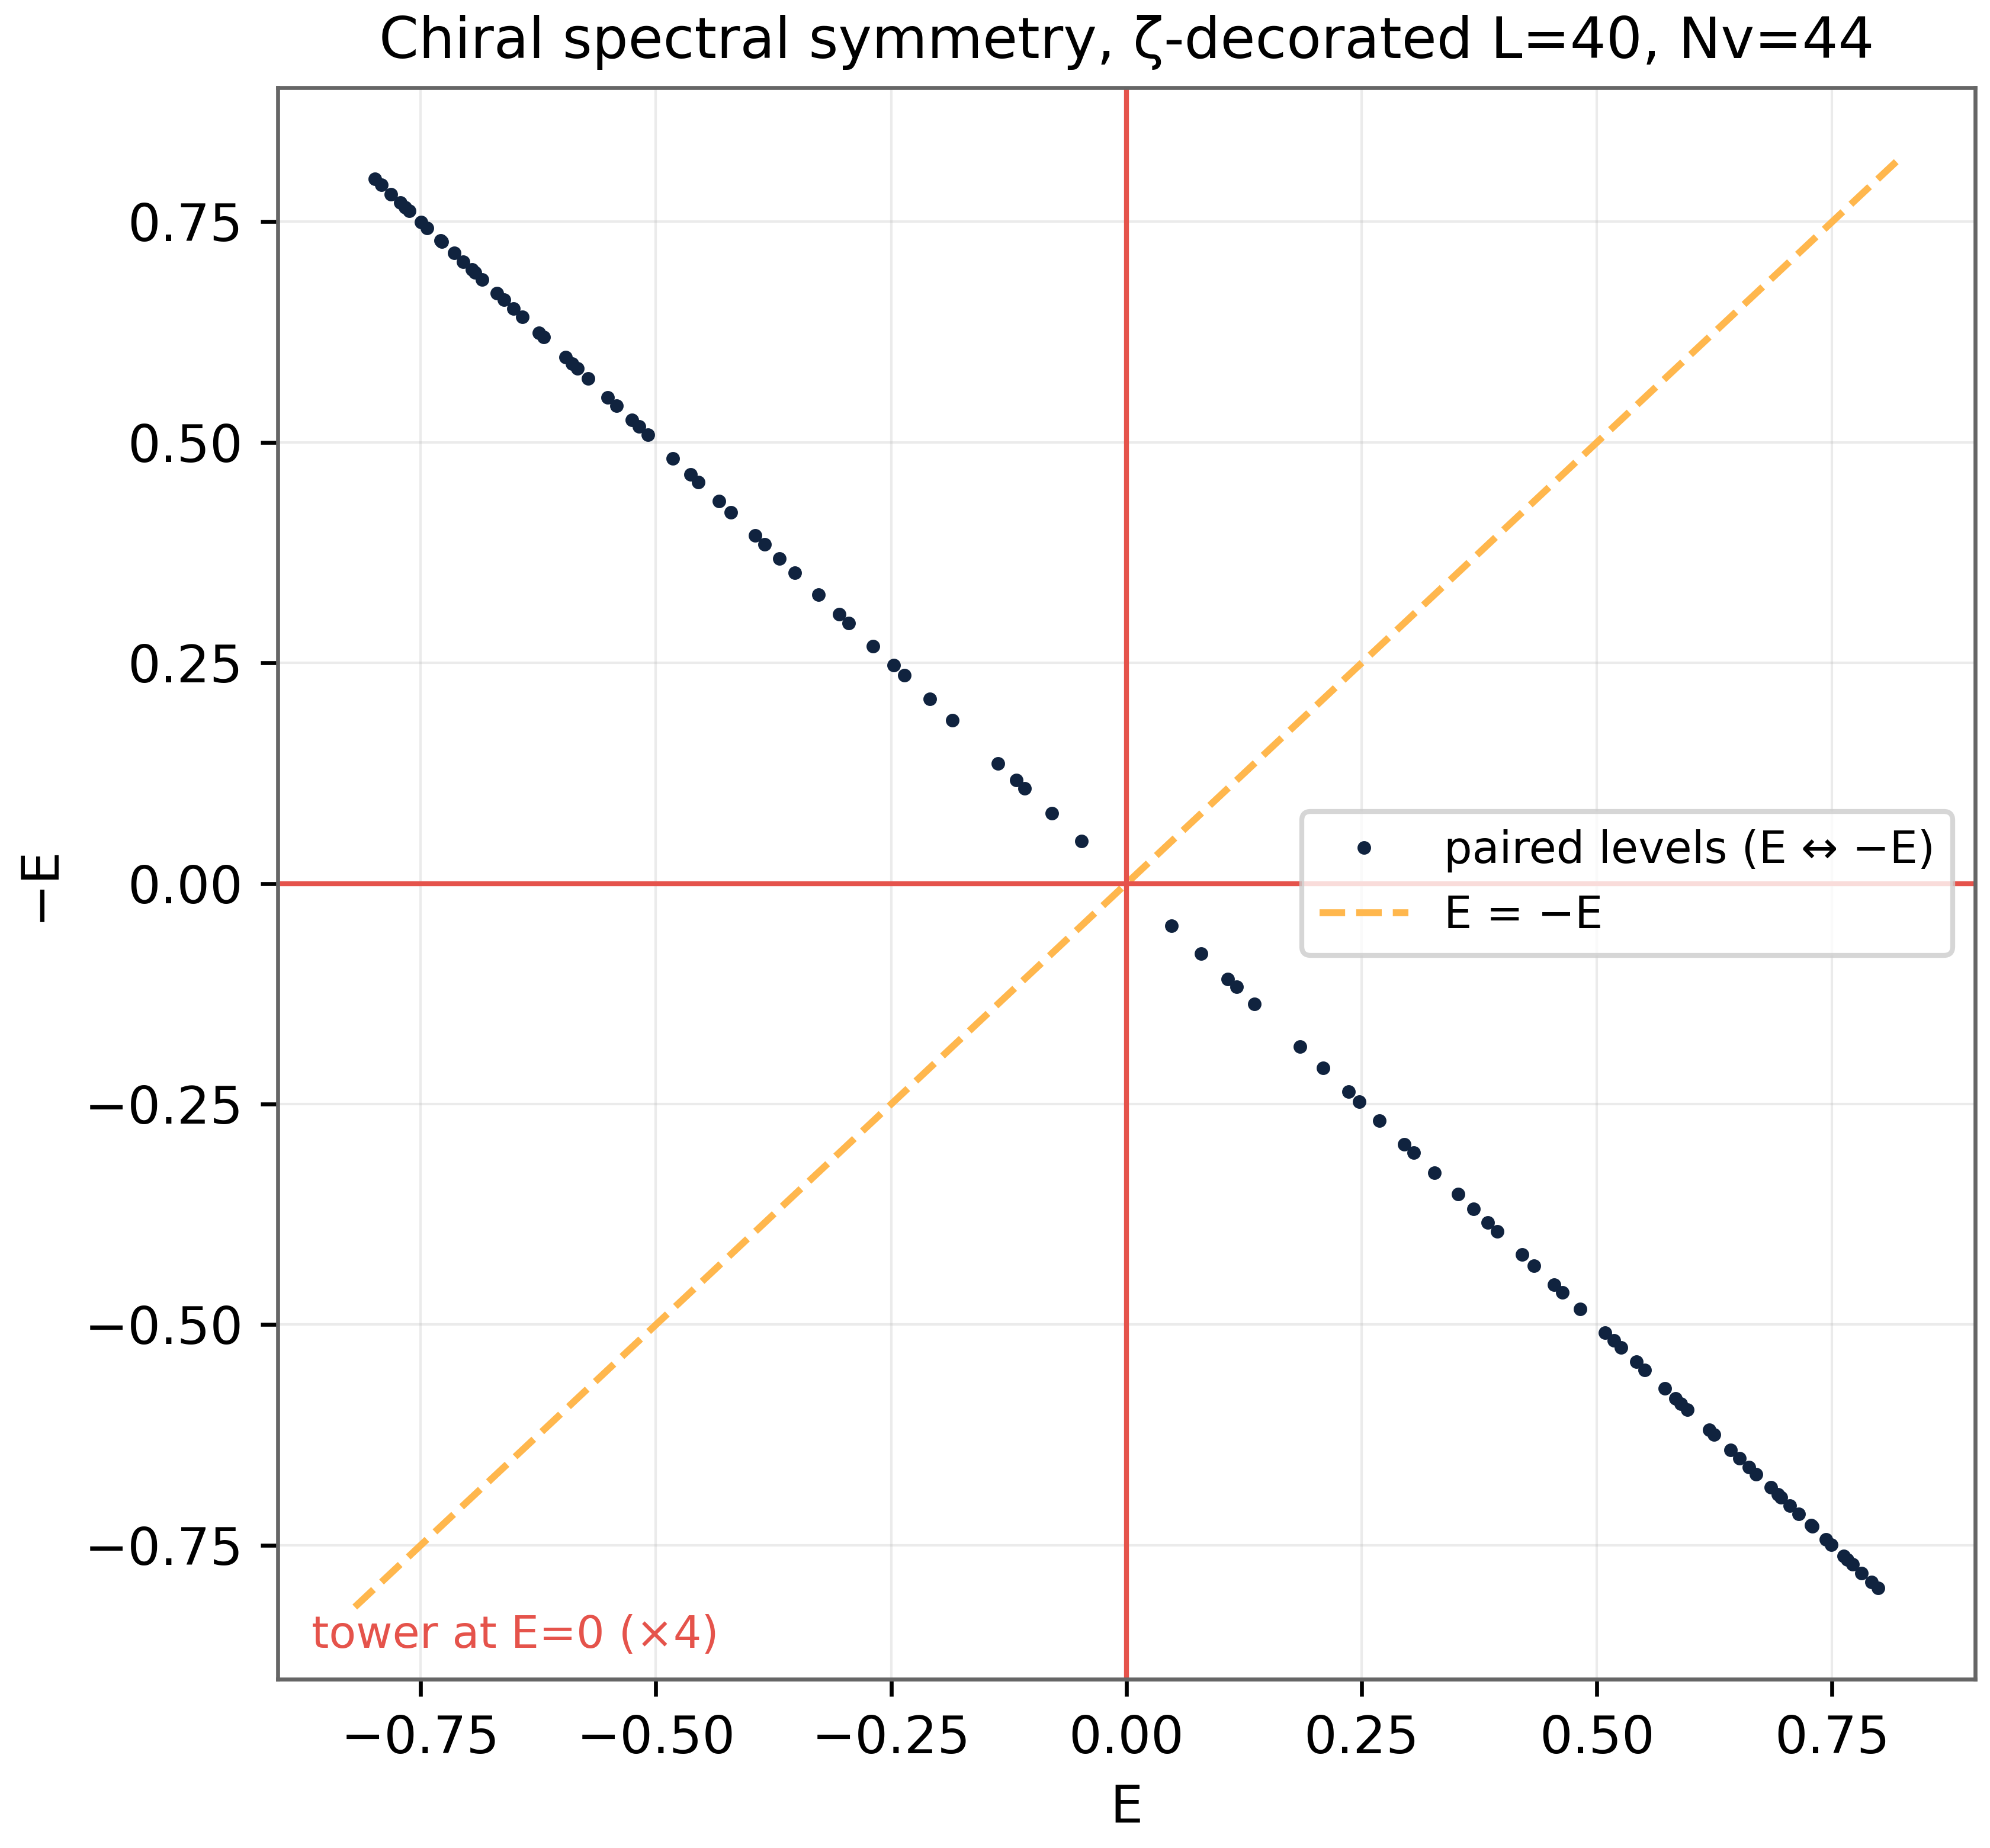
\includegraphics[max width=\columnwidth, max height=0.42\textheight]{figures/fig_D8_chiral_symmetry.png}
\caption{Canonical D8 figure (600 dpi): the pairing audit and valley structure, produced by the original harness.}\label{fig:d8_1}
\end{figure}
\begin{figure}[htbp]\centering
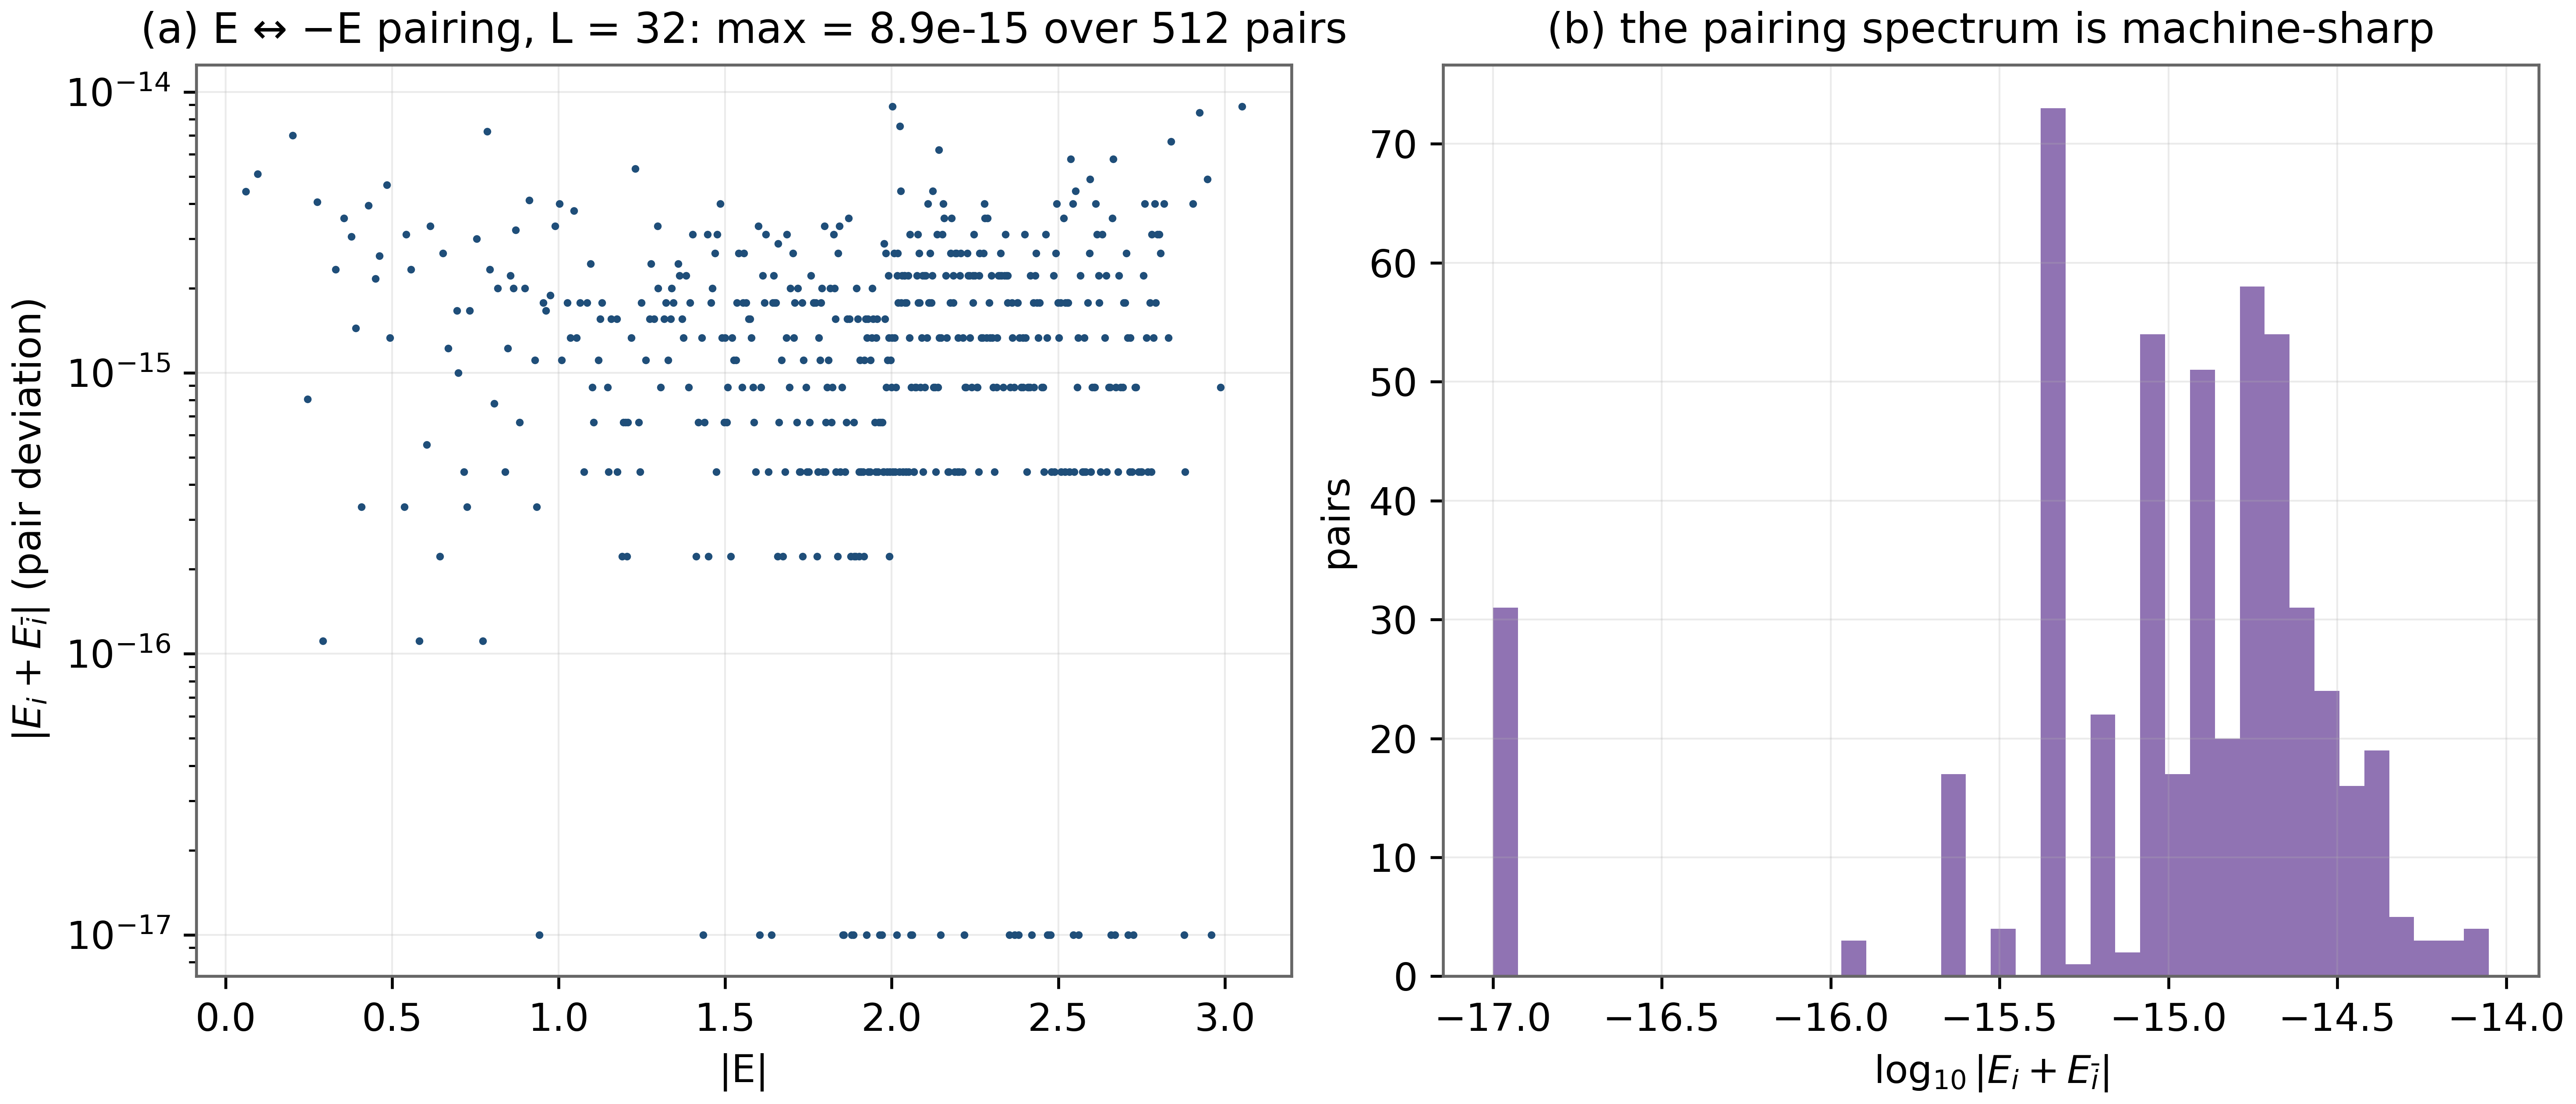
\includegraphics[max width=\columnwidth, max height=0.42\textheight]{figures/d08_extra_pairing.png}
\caption{Companion panels (recomputed at $L=32$, canonical modules and seed): (a) pair deviation $|E_i + E_{\bar i}|$ vs $|E_i|$ on a log axis -- every pair at machine depth; (b) the pairing-deviation histogram.}\label{fig:d8_2}
\end{figure}

\section{Discussion}
D8 is the laboratory's symmetry keystone. Every later test that claims machine precision for a protected quantity -- the wall mode of D9, the chiral-breaking law of D13 -- stands on the exact anticommutation verified here. Equally, the explicit demonstration that symmetry and index are different currencies (one survives decoration, one does not) is the conceptual preparation for the Jackiw--Rossi programme: protection must be engineered where the index is, not merely asserted where the symmetry is.

Extensions should treat D8 as a required audit gate: any new decoration, gauge or regularization must reproduce $\|\{H,\Gamma\}\| = 0$ and the pairing law before its statistics can be interpreted. A decoration that fails the audit has changed symmetry class, and the random-matrix comparison targets change with it.

\section{Reproducibility}
\begin{itemize}[leftmargin=1.2em, itemsep=0.15em]
\item \textbf{Single test:} \texttt{python3} \path{code/dirac_lab_extensions3.py} \texttt{--test D8} (add \texttt{--quick} for a reduced pass; \texttt{--no-figures} to skip the 600-dpi figure).
\item \textbf{Canonical run:} \texttt{make all} regenerates the whole D1--D14 ledger into \path{results/}; this monograph's ledger is the verbatim per-check table of that run.
\item \textbf{Determinism:} seed 96 (parent convention); the $\zeta$ tables are the Odlyzko-derived files in \path{data/} with provenance in their headers.
\item \textbf{Figures:} the canonical figure was regenerated into this folder by the v1.4 harness (the original test function itself); companion panels are recomputed with the same modules (\path{scripts/make_extra_figures.py}). All figures are 600 dpi.
\item \textbf{Cross-verification:} \texttt{julia} \path{code/dirac_lab_cross.jl} re-derives this test's verdicts from the written conventions alone (see \path{results/CROSS_VERIFICATION.md}).
\item \textbf{Artifacts in this folder:} \path{monograph.tex} (this document's source), \path{results.json} (machine-readable ledger), \path{figures/} (600-dpi figures), and the canonical CSV of the test.
\end{itemize}

\section*{References}
\begin{thebibliography}{99}\small
\bibitem{mecklenburgshen} C. L. Kane and E. J. Mele, Quantum spin Hall effect in graphene, Phys. Rev. Lett. 95, 226801 (2005). See also A. C. Neto et al., The electronic properties of graphene, Rev. Mod. Phys. 81, 109 (2009).
\bibitem{atyahbott} M. F. Atiyah and R. Bott, The Yang--Mills equations over Riemann surfaces, Philos. Trans. R. Soc. A 308, 523 (1983).
\bibitem{jackiwrebbi} R. Jackiw and C. Rebbi, Solitons with fermion number $1/2$, Phys. Rev. D 13, 3398 (1976).
\bibitem{jackiwrossi} R. Jackiw and P. Rossi, Zero modes of the vortex--fermion system, Nucl. Phys. B 190, 681 (1981).
\end{thebibliography}

\vfill
\noindent\rule{\textwidth}{0.4pt}\\[0.2em]
{\footnotesize\color{labgray} AB-Cloud Dirac Laboratory · per-test monograph series v1.4 · compiled with Tectonic (LaTeX) · all numbers traceable to \texttt{results/run\_20261006\_full\_v13} · \texttt{D8} of 14.}

\end{document}